\documentclass[11pt,a4paper]{article}

\usepackage{fontspec}
\usepackage{amsmath,amssymb}
\usepackage{booktabs}
\usepackage{graphicx}
\usepackage{caption}
\usepackage{xcolor}
\usepackage[ruled,vlined,linesnumbered]{algorithm2e}
\usepackage[a4paper,margin=1.75cm]{geometry}
\usepackage{titlesec}
\titlespacing*{\section}{0pt}{6pt}{2pt}
\titlespacing*{\subsection}{0pt}{5pt}{1pt}
\titleformat{\section}{\large\bfseries\color{navy}}{\thesection}{0.6em}{}
\titleformat{\subsection}{\normalsize\bfseries\color{navy}}{\thesubsection}{0.5em}{}

\graphicspath{{figures/}}
\captionsetup{font=small,labelfont=bf}
\renewcommand{\figurename}{Şekil}
\renewcommand{\tablename}{Tablo}
\SetAlgorithmName{Algoritma}{Algoritma}{Algoritma Listesi}
\SetKwProg{Fn}{fonksiyon}{:}{}
\setlength{\parindent}{0pt}
\setlength{\parskip}{2.5pt}
\definecolor{navy}{HTML}{1F3A5F}
\newcommand{\code}[1]{\texttt{\small #1}}

\title{\vspace{-1.2cm}\textbf{\color{navy} Thread Tabanlı Convex (Dışbükey) Poligon Kontrolü}\\[2pt]
\large Çapraz Çarpım Tabanlı Konvekslik Testinin Java İş Parçacıkları ile Paralelleştirilmesi}
\author{Duha Keskin (22360859003) \quad Yunus Alim Avşar (23360859710)}
\date{Paralel Programlama --- Haziran 2026}

\begin{document}
\maketitle
\vspace{-0.6cm}

\begin{abstract}\noindent\small
Düzlemde sıralı $(x,y)$ koordinatlarından oluşan bir nokta dizisinin kapalı bir convex
poligon oluşturup oluşturmadığını saptayan, Java \code{java.util.concurrent} altyapısıyla
paralelleştirilmiş bir program sunulmaktadır. Konvekslik, ardışık üçlülerin çapraz çarpım
\emph{işareti} ile birlikte işaretli dış açıların toplamının $\pm2\pi$ olması koşuluyla
\emph{tam-doğru} biçimde test edilir; bu sayede pentagram gibi kendiyle kesişen poligonlar da
doğru reddedilir. İş yükü, paylaşılan bir \code{ExecutorService} havuzu üzerinde çekirdek
sayısı kadar parçaya bölünür ve sonuçlar kilit kullanılmadan bir \emph{reduction} ile
birleştirilir. Apple M3 Pro (12 çekirdek) üzerinde, $N=10^{7}$ nokta için \textbf{6.33$\times$}
hızlanma ve thread sayısına göre $E=S/C$ verimliliğinin performans çekirdeği sınırında düşüşü
ölçülmüş; sonuçlar Amdahl Yasası ve Karp--Flatt seri-pay metriğiyle yorumlanmıştır.
\end{abstract}

\section{Problemin Tanımı}
Sıralı $(x_i,y_i)$, $i=0,\dots,n-1$ köşelerinden oluşan kapalı bir poligonun
\textbf{convex} (dışbükey) olup olmadığını belirlemek istiyoruz. Çözüm hem \textbf{tek thread
(seri)} hem de \textbf{çok thread (paralel)} olarak gerçeklendi; iki sürümün süreleri ölçülerek
hızlanma katsayısı hesaplandı. Problem, çarpışma denetimi, robot hareket planlama ve CBS gibi
alanlarda temel bir geometrik yordamdır ve birazdan görüleceği gibi \emph{veri-paralel} bir
yapıya sahiptir.

\section{Algoritma ve Çalışma Prensibi}

\subsection{Çapraz çarpım ve dönüş yönü}
Ardışık üç köşe $P_i,P_{i+1},P_{i+2}$ için dönüş yönü, gelen kenar
$\vec{e}_i=P_{i+1}-P_i$ ile giden kenar $\vec{e}_{i+1}=P_{i+2}-P_{i+1}$ çapraz çarpımının
$z$ bileşeni (bir $2\times2$ determinant) ile bulunur:
\begin{equation}
z_i=\det\!\begin{pmatrix} x_{i+1}-x_i & x_{i+2}-x_{i+1}\\[2pt] y_{i+1}-y_i & y_{i+2}-y_{i+1}\end{pmatrix}
=(x_{i+1}-x_i)(y_{i+2}-y_{i+1})-(y_{i+1}-y_i)(x_{i+2}-x_{i+1}).
\end{equation}
\begin{equation}
\text{d\"on\"u\c{s}}(P_{i+1})=
\begin{cases}
\text{sola (saat yönü tersi)} & z_i>0,\\
\text{sağa (saat yönü)}       & z_i<0,\\
\text{doğrusal (collinear)}   & z_i=0.
\end{cases}
\end{equation}
İndisler $\bmod\,n$ alınır; böylece kapanış üçlüleri $(P_{n-1},P_0,P_1)$ ve $(P_{n-2},P_{n-1},P_0)$
de denetlenir.

\subsection{Gerekli \emph{ve} yeterli koşul}
``Tüm $z_i$ aynı işaretli'' koşulu konvekslik için \textbf{gerekli ama yeterli değildir}:
Şekil~\ref{fig:shapes}'teki pentagram (yıldız) tüm dönüşleri aynı yönde olduğu hâlde kendiyle
kesişir ve convex değildir. Yeterlilik için poligonun sınırının \emph{tam bir kez} dolandığını,
yani işaretli dış (dönüş) açılarının toplamının $\pm2\pi$ olduğunu da doğrularız:
\begin{equation}
\theta_i=\operatorname{atan2}\!\big(z_i,\;\vec{e}_i\cdot\vec{e}_{i+1}\big),\qquad
\textbf{convex}\iff
\underbrace{\big(\operatorname{sgn} z_i \text{ sabit}\big)}_{\text{tek dönüş yönü}}\ \wedge\
\underbrace{\Big|\textstyle\sum_{i=0}^{n-1}\theta_i\Big|=2\pi}_{\text{tek tur}} .
\label{eq:convex}
\end{equation}
Buna göre basit convex poligonda toplam $\pm2\pi$, pentagramda $\pm4\pi$, $180^\circ$ geri-dönüş
(spike) veya tüm-doğrusal dejenere girdilerde ise $2\pi$'den sapar ve doğru biçimde reddedilir.
Açı toplamı $\sum\theta_i$ bir \emph{toplama} olduğundan, çapraz çarpım işareti ile birlikte
veri-paralel olarak hesaplanabilir.

\begin{figure}[t]
\centering
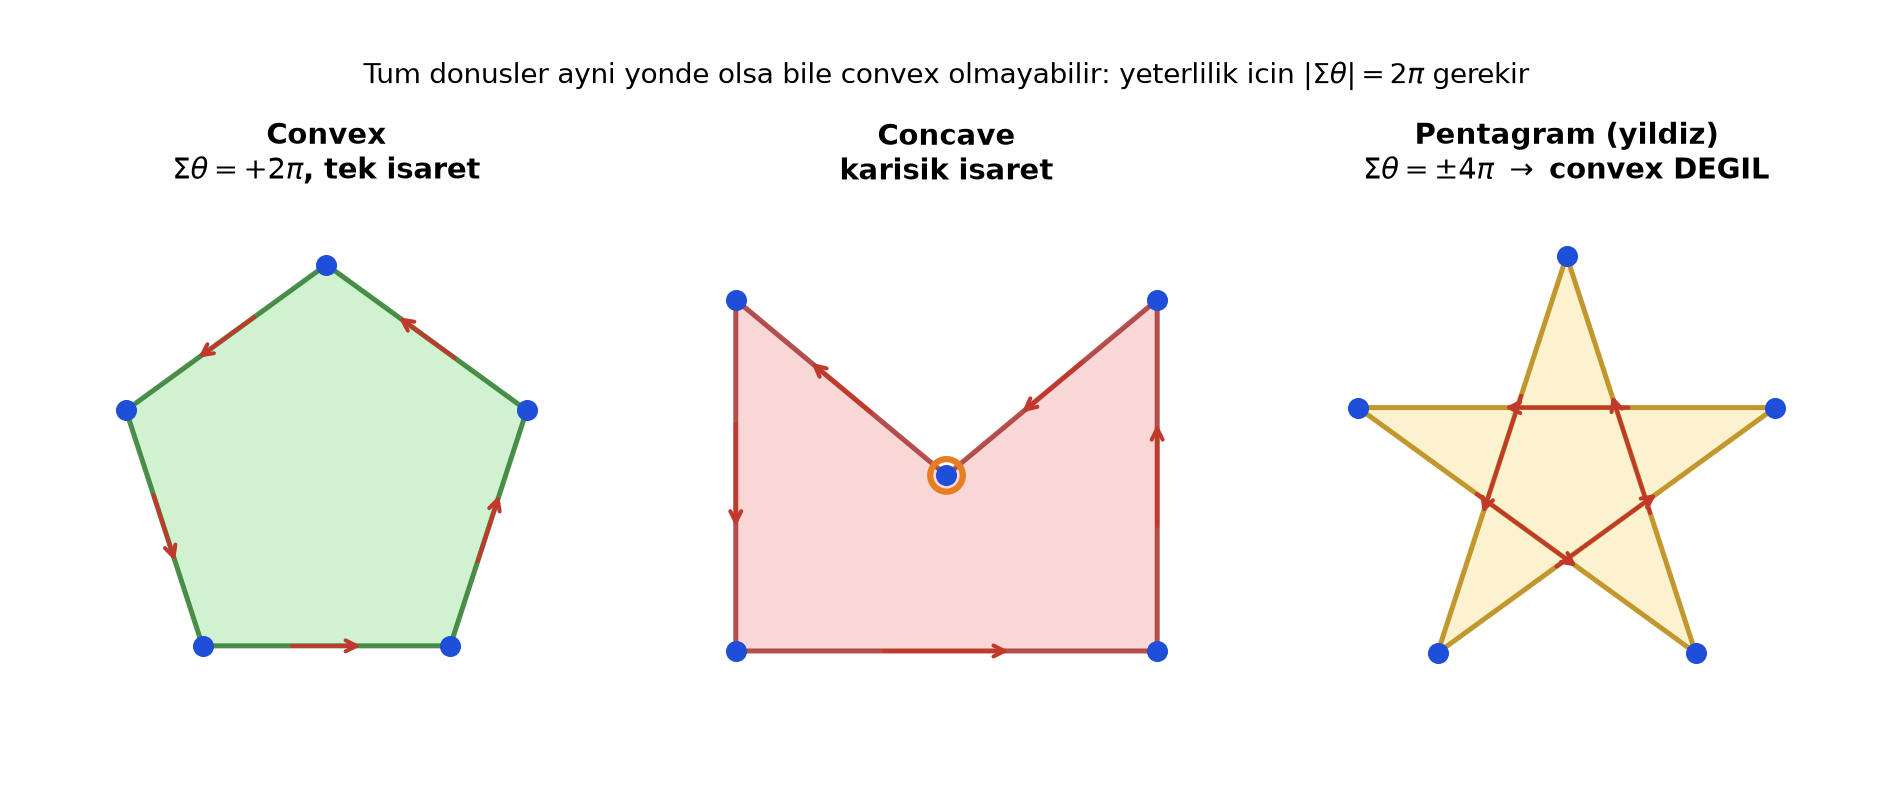
\includegraphics[width=\linewidth]{fig1_convex_vs_concave.png}
\caption{Üç örnek: \textbf{(sol)} convex beşgen $\Sigma\theta=+2\pi$; \textbf{(orta)} concave
``V'' örneği, karışık işaret; \textbf{(sağ)} pentagram, tüm dönüşler aynı yönde ama
$\Sigma\theta=\pm4\pi$ ve kendiyle kesişen $\Rightarrow$ convex değil.}
\label{fig:shapes}
\end{figure}

\subsection{Sınıflar ve fonksiyonlar}
Proje OOP ilkeleriyle dört dosyaya ayrıldı:
\begin{itemize}\setlength\itemsep{1pt}
\item \code{Point} --- salt veri sınıfı ($x,y$ çiftini tutar).
\item \code{ChunkResult} --- bir alt-aralığın reduction sonucu: $(\,\mathrm{sign},\,\mathrm{turnSum},\,\mathrm{mixed}\,)$.
\item \code{ConvexCheckerTask implements Callable<ChunkResult>} --- verilen $[\text{start},\text{end})$ aralığındaki üçlüler için çapraz çarpım işaretini \emph{ve} işaretli açı toplamını tek geçişte üretir.
\item \code{Main} --- veri üretimi, paylaşılan havuz, ölçüm, \code{decide()} birleştirme ve CSV çıktısı.
\end{itemize}

\subsection{Çalışma örnekleri}
\code{generateConvexPolygon(5)}, yarıçapı 100 olan çember üzerinde
$(100,0),(30.9,95.1),(-80.9,58.8),(-80.9,-58.8),(30.9,-95.1)$ noktalarını üretir; tüm $z_i>0$ ve
$\Sigma\theta=2\pi \Rightarrow$ \textbf{convex}. \code{makeConcaveSample()} ise
$(0,0),(4,0),(4,4),(2,2),(0,4)$ döndürür; $(4,4)\!\to\!(2,2)\!\to\!(0,4)$ üçlüsü ters döner
(karışık işaret) $\Rightarrow$ \textbf{convex değil}. \code{makePentagram()} beş çember
noktasını yıldız sırasında dolaşır; tek işaret ama $\Sigma\theta=4\pi \Rightarrow$
\textbf{convex değil}. Tüm bu durumlar programın doğruluk testlerinde otomatik denetlenir.

\section{Paralel Çözüm}

\subsection{İşin bölünmesi (data decomposition)}
$N$ noktalık dizi, $C=\code{Runtime.getRuntime().availableProcessors()}$ adet çekirdeğe
yaklaşık eşit chunk'lara ayrılır:
\begin{equation}
\text{chunk}_k=\big[k\lfloor N/C\rfloor,\ (k{+}1)\lfloor N/C\rfloor\big),\ k=0,\dots,C{-}2;
\qquad \text{chunk}_{C-1}=\big[(C{-}1)\lfloor N/C\rfloor,\ N\big).
\end{equation}
Son chunk kalan elemanları sahiplenir; hiçbir köşe atlanmaz veya iki kez sayılmaz. İndis $i$'ye
ait dönüş tam olarak bir chunk'a düştüğü için $N$ köşenin tamamı \emph{tam bir kez} işlenir.

\begin{algorithm}[t]
\DontPrintSemicolon
\KwIn{Noktalar $P=\langle P_0,\dots,P_{N-1}\rangle$; çekirdek sayısı $C$; paylaşılan havuz \texttt{pool}}
\KwOut{poligon convex mi? (doğru/yanlış)}
\If{$N<3$}{\Return \textbf{hata} (en az 3 nokta gerekir)\;}
$\mathrm{futures}\leftarrow$ boş liste\;
\For{$k\leftarrow 0$ \KwTo $C-1$}{
  $(\mathrm{start},\mathrm{end})\leftarrow \mathrm{chunk}_k$\;
  futures'a \texttt{pool.submit(}\,\textsc{ChunkScan}$(P,\mathrm{start},\mathrm{end})$\texttt{)} ekle\;
}
$R\leftarrow$ tüm \texttt{future.get()} sonuçları\tcp*{örtük senkronizasyon}
\Return \textsc{Decide}$(R)$\;
\BlankLine
\Fn{\textsc{ChunkScan}$(P,\mathrm{start},\mathrm{end})$}{
  $\mathrm{sign}\leftarrow0$;\ $\tau\leftarrow0$\;
  \For{$i\leftarrow\mathrm{start}$ \KwTo $\mathrm{end}-1$}{
    $z\leftarrow$ çapraz çarpım;\quad $\tau\leftarrow\tau+\operatorname{atan2}\!\big(z,\ \vec{e}_i\cdot\vec{e}_{i+1}\big)$\;
    işaret tutarlılığını güncelle; karışık işaret görülürse \textbf{mixed}\;
  }
  \Return $(\mathrm{sign},\tau,\mathrm{mixed})$\;
}
\Fn{\textsc{Decide}$(R)$}{
  $\Sigma\tau\leftarrow\sum_{r\in R} r.\tau$\;
  \lIf{mixed var / işaretler çelişir / hiç işaret yok}{\Return \textbf{yanlış}}
  \Return $\big|\,|\Sigma\tau|-2\pi\,\big|<\varepsilon$\;
}
\caption{Paralel Konvekslik Kontrolü (decomposition + reduction)}
\label{alg:main}
\end{algorithm}

\subsection{Thread havuzu ve kilitsiz birleştirme}
\code{new Thread()} yerine \emph{tek bir} \code{Executors.newFixedThreadPool} havuzu programda bir
kez kurulur ve \emph{tüm} ölçümlerde yeniden kullanılır; böylece havuz kurulum/yıkım maliyeti
ölçülen pencerenin dışında kalır (bkz.\ \S\ref{sec:method}). Her görev \code{submit()} ile
gönderilir, \code{Future.get()} örtük senkronizasyon sağlar. Thread'ler \textbf{paylaşılan bir
değişkene yazmaz}; her biri yerel sayaç ve yerel açı toplamı tutup tek bir \code{ChunkResult}
döndürür. Bu yüzden \code{synchronized}, \code{Lock} veya \code{Atomic*} gibi primitiflere gerek
kalmaz; kilit çekişmesi sıfırdır. Nihai karar (Denklem~\ref{eq:convex}) \code{Main.decide()}
içinde bir \emph{reduction} ile verilir: işaret tutarlılığı kontrol edilir ve kısmî açı
toplamları $\Sigma\theta$'ya eklenir.

\textbf{Klasik tuzak.} Her thread'in yalnızca kendi chunk'ı içinde ``convex mi?'' kararı vermesi
hatalıdır: A chunk'ı hep sola, B chunk'ı hep sağa dönerse ikisi de bağımsızca ``convex'' der.
Bu projede thread'ler yalnızca \emph{işaret + açı} döndürür; küresel kararı \code{decide()} verir.

\section{Deneysel Kurulum}\label{sec:method}

\begin{table}[h]
\centering\small
\begin{tabular}{@{}ll@{}}
\toprule
\textbf{Bileşen} & \textbf{Değer}\\
\midrule
İşlemci & Apple M3 Pro --- 12 çekirdek (6 performans + 6 verim), tek soket\\
Bellek / OS & 18 GB birleşik bellek; macOS 26.4.1 (arm64)\\
JDK / JVM & OpenJDK 21.0.10 (JetBrains Runtime), \code{-Xmx4g}\\
Zamanlama & \code{System.nanoTime()} (monotonik, ns çözünürlük)\\
Yöntem & boyut başına 10 ısınma + 15 ölçüm; \textbf{medyan} + min + std\\
DCE koruması & sonuç \code{volatile} bir sink'e işlenir (JIT ölü-kod elemesi engellenir)\\
\bottomrule
\end{tabular}
\caption{Deney ortamı ve ölçüm metodolojisi. Tüm sayılar tek bir koşunun
\code{results.csv}/\code{results\_threads.csv} çıktısından alınmıştır; ondalık ayraç noktadır.}
\label{tab:env}
\end{table}

JVM'in dinamik JIT derleyicisi nedeniyle her boyut için önce 10 ısınma turu (zamanlanmaz)
koşulur; ardından 15 ölçümün \textbf{medyanı} alınır (tek bir GC duraklamasına karşı ortalamadan
daha dayanıklıdır). Sonuçlar bir sink'te tüketildiği için derleyici döngüyü ölü-kod olarak
eleyemez. \code{generateConvexPolygon} maliyeti zamanlanan pencerenin dışındadır ve $10^{7}$'lik
poligon yalnızca bir kez üretilir.

\section{Deneysel Sonuçlar}

Hızlanma ve verimlilik:
\begin{equation}
S=\frac{T_{\text{seri}}}{T_{\text{paralel}}},\qquad E=\frac{S}{C}.
\end{equation}

\begin{table}[h]
\centering\small
\begin{tabular}{@{}rrrrrc@{}}
\toprule
$N$ & $T_{\text{seri}}$ (ms) & $T_{\text{paralel}}$ (ms) & $S$ & $E=S/C$ & Convex?\\
\midrule
1\,000        & 0.024  & 0.073  & 0.33$\times$ & \%3  & evet\\
10\,000       & 0.088  & 0.065  & 1.35$\times$ & \%11 & evet\\
100\,000      & 0.867  & 0.239  & 3.63$\times$ & \%30 & evet\\
1\,000\,000   & 8.198  & 1.453  & 5.64$\times$ & \%47 & evet\\
5\,000\,000   & 41.58  & 6.79   & 6.12$\times$ & \%51 & evet\\
10\,000\,000  & 82.64  & 13.05  & \textbf{6.33$\times$} & \%53 & evet\\
\bottomrule
\end{tabular}
\caption{Veri büyüklüğüne göre süreler, hızlanma ($C=12$ thread) ve verimlilik.}
\label{tab:sizes}
\end{table}

\begin{figure}[h]
\centering
\begin{minipage}{0.495\linewidth}\centering
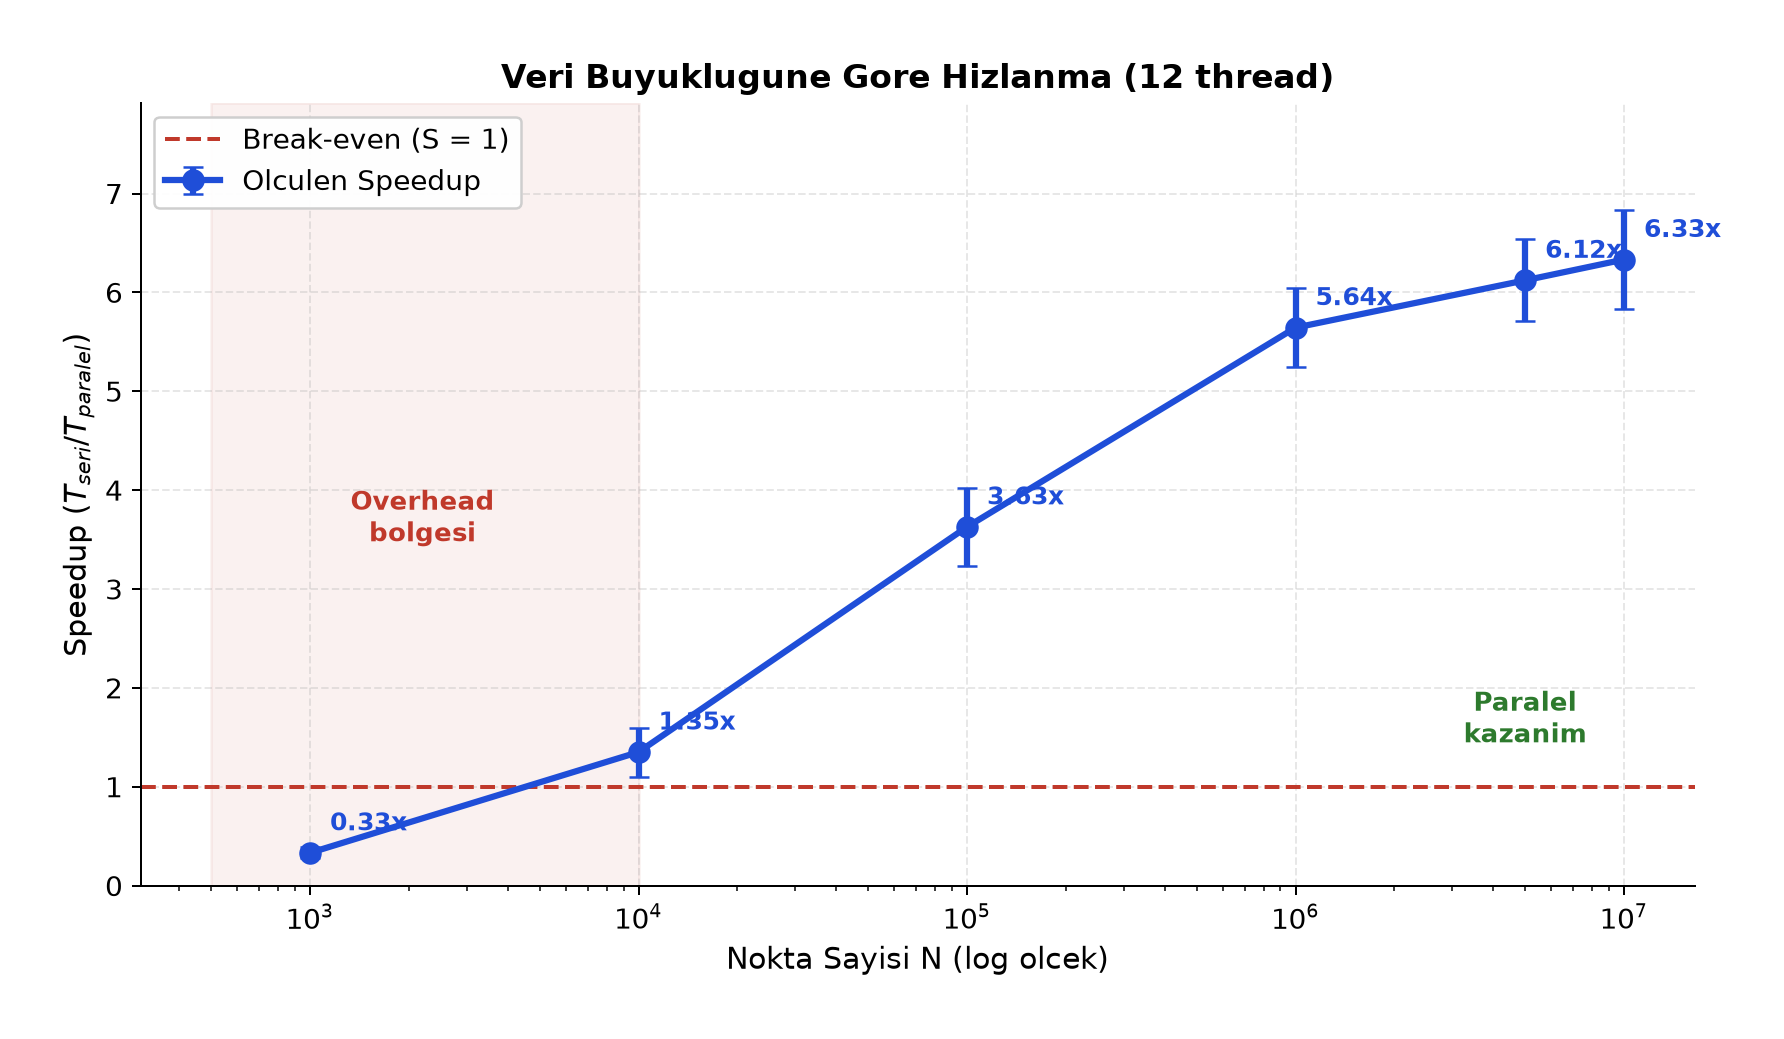
\includegraphics[width=\linewidth]{fig2_speedup_vs_n.png}
\end{minipage}\hfill
\begin{minipage}{0.495\linewidth}\centering
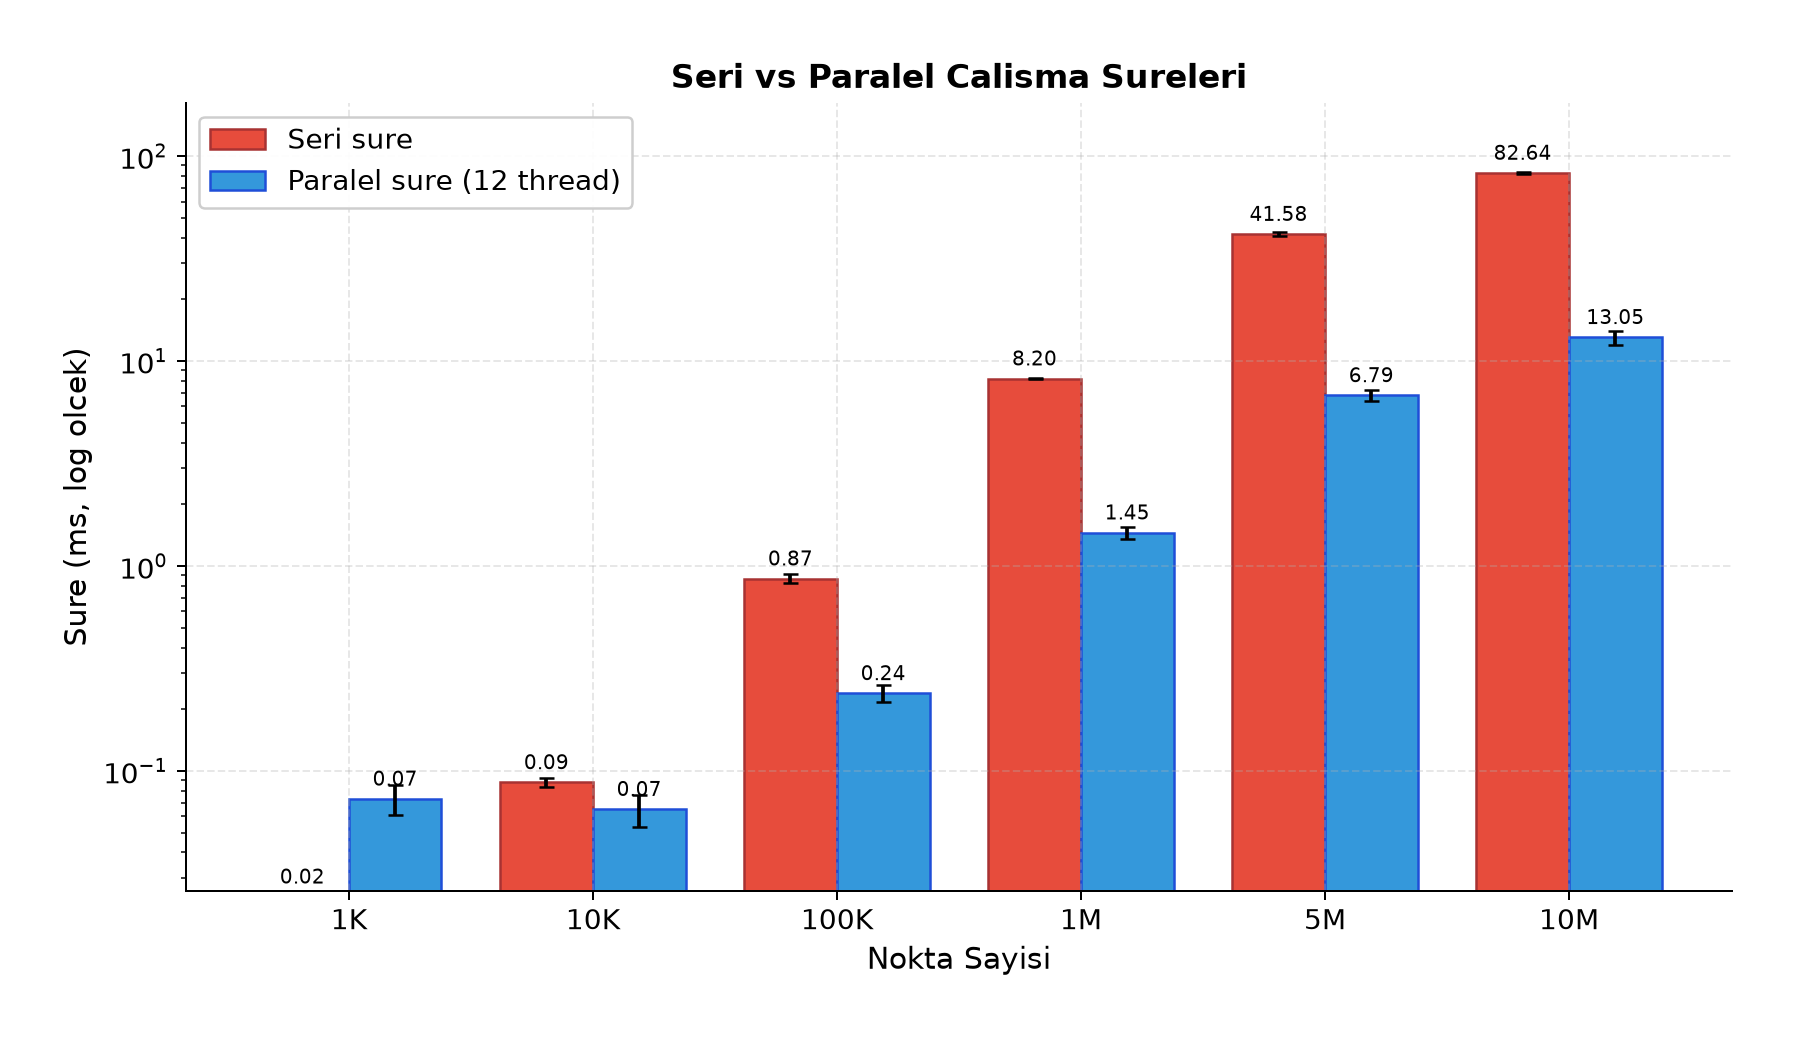
\includegraphics[width=\linewidth]{fig3_times_bar.png}
\end{minipage}
\caption{\textbf{(sol)} $N$'ye göre Speedup (yarı-log, hata çubuklu): kırılma noktası
$N=10^{4}$. \textbf{(sağ)} Seri vs paralel süreler (log-$y$).}
\label{fig:sizes}
\end{figure}

\begin{table}[h]
\centering\small
\begin{tabular}{@{}rrrrrr@{}}
\toprule
$C$ (thread) & $T_{\text{seri}}$ (ms) & $T_{\text{paralel}}$ (ms) & $S$ & $E=S/C$ & Karp--Flatt $e$\\
\midrule
1  & 86.35 & 85.39 & 1.01$\times$ & \%101 & ---\\
2  & 88.38 & 44.41 & 1.99$\times$ & \%99  & 0.005\\
4  & 84.44 & 21.89 & 3.86$\times$ & \%96  & 0.012\\
6  & 87.06 & 20.02 & 4.35$\times$ & \%72  & 0.076\\
8  & 83.77 & 17.30 & 4.84$\times$ & \%61  & 0.093\\
12 & 82.20 & 12.77 & \textbf{6.43$\times$} & \%54 & 0.079\\
16 & 87.79 & 14.33 & 6.13$\times$ & \%38 & 0.107\\
\bottomrule
\end{tabular}
\caption{Sabit $N=10^{7}$ için thread sayısına göre ölçeklenme. $C=16$ aşırı-abonelik
(oversubscription); makinede yalnızca 12 çekirdek vardır.}
\label{tab:threads}
\end{table}

\begin{figure}[h]
\centering
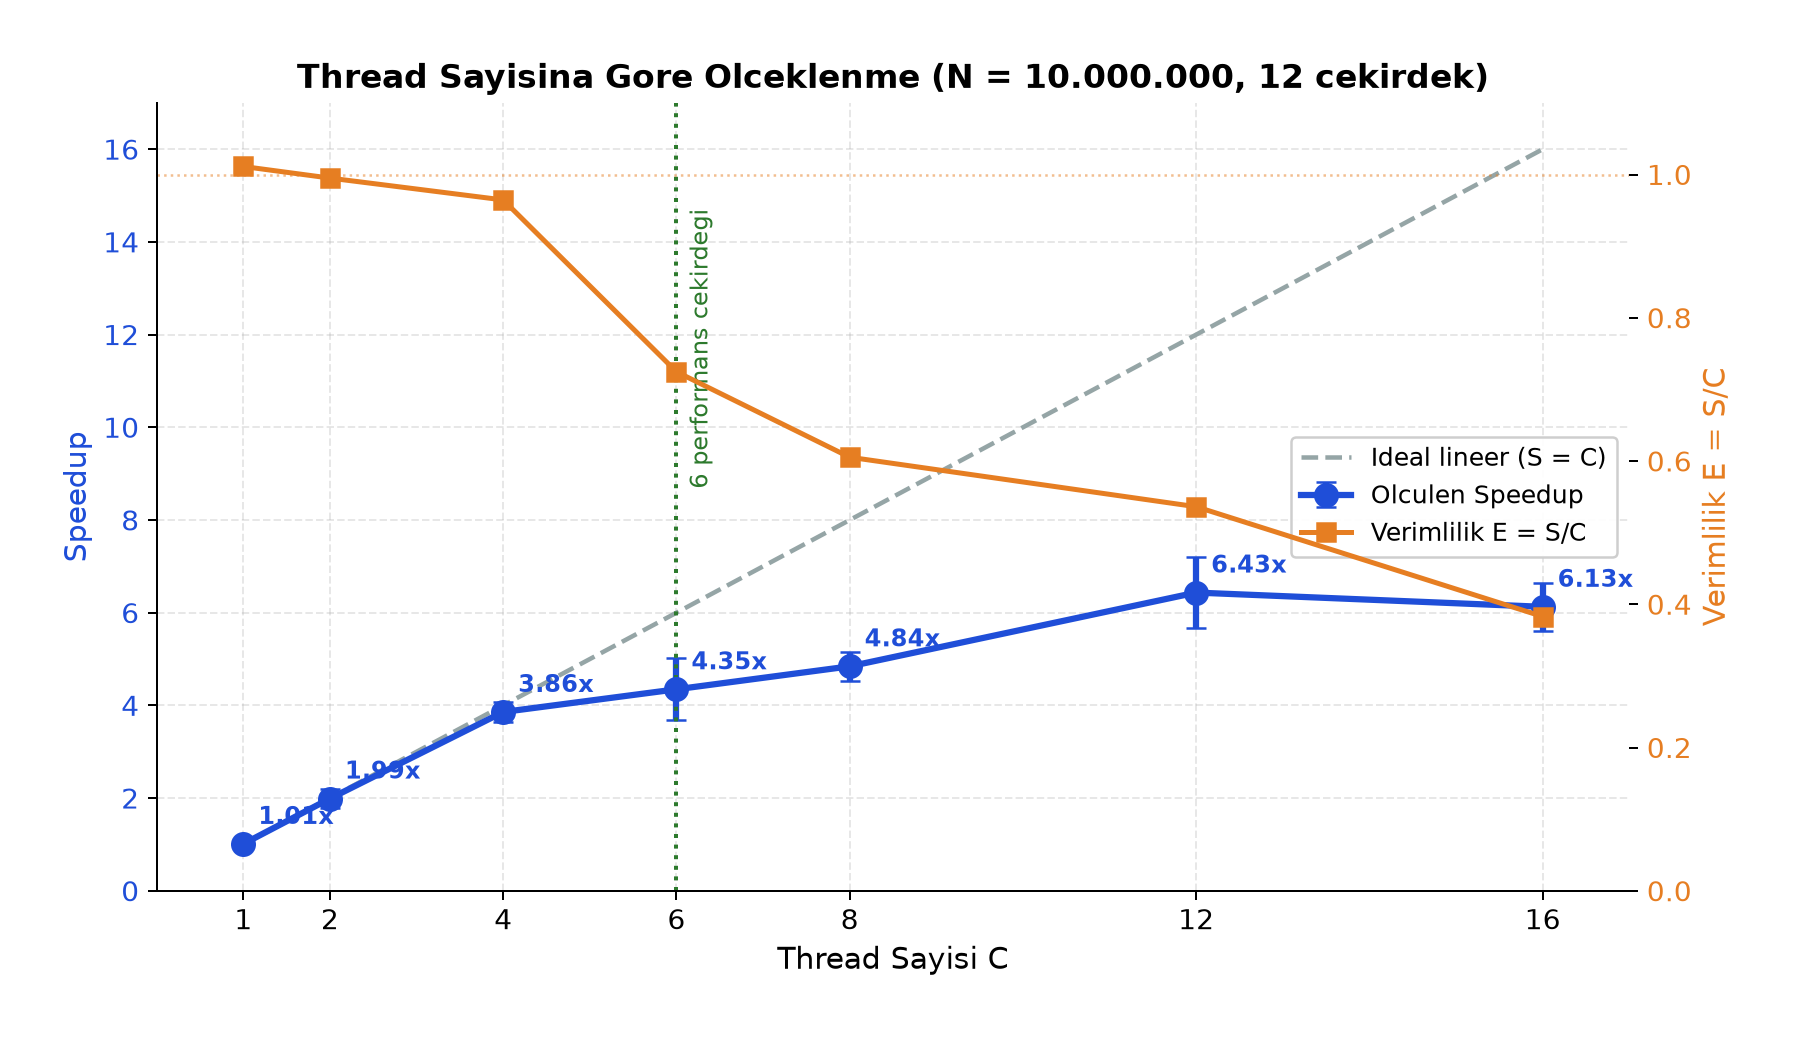
\includegraphics[width=0.62\linewidth]{fig4_speedup_vs_threads.png}
\caption{Thread sayısına göre Speedup (mavi) ve verimlilik $E=S/C$ (turuncu, sağ eksen).
Verimlilik 4 thread'e kadar $\approx1$; 6 performans çekirdeği sınırından (yeşil çizgi) sonra
düşer.}
\label{fig:threads}
\end{figure}

\textbf{Hangi parametrede ne kadar hızlanma?} Sabit $C=12$ için
$N{=}10^{4}\!\to\!1.35\times$, $N{=}10^{5}\!\to\!3.63\times$, $N{=}10^{6}\!\to\!5.64\times$,
$N{=}10^{7}\!\to\!6.33\times$. Sabit $N{=}10^{7}$ için
$C{=}2\!\to\!1.99\times$, $C{=}4\!\to\!3.86\times$, $C{=}8\!\to\!4.84\times$,
$C{=}12\!\to\!6.43\times$.

\section{Analiz}

\paragraph{Küçük $N$ ve kırılma noktası.} $N\le10^{3}$ için $S<1$: \code{submit}/\code{get}
koordinasyonunun sabit maliyeti, küçük iş yükünden büyüktür. Havuz \emph{yeniden kullanıldığı}
için bu maliyet yalnızca koordinasyondur (havuz kurulumu değil) ve kırılma noktası daha
$N=10^{4}$'te aşılır; bu noktadan sonra paralel sürüm üstünlüğe geçer (Şekil~\ref{fig:sizes}).

\paragraph{Amdahl ve Karp--Flatt.} Programın seri kalan payı $s$ ise teorik üst sınır
\begin{equation}
S_{\max}(C)=\frac{1}{\,s+\dfrac{1-s}{C}\,}.
\end{equation}
Seri payı veriden kestirmek için Karp--Flatt metriği kullanılır:
\begin{equation}
e=\frac{\dfrac{1}{S}-\dfrac{1}{C}}{\,1-\dfrac{1}{C}\,}.
\end{equation}
Tablo~\ref{tab:threads}'te $e$, 4 thread'e kadar $\approx0.01$ (neredeyse ideal) iken $C\ge6$'da
$\sim0.08$--$0.11$'e yükselir. Bu \emph{sabit olmayan, artan} seri pay klasik bir bellek/iletişim
darboğazı değil, \textbf{heterojen çekirdek} etkisidir: M3 Pro 6 \emph{performans} + 6 \emph{verim}
çekirdeği barındırır. İlk $\sim6$ thread hızlı P-çekirdeklerine yerleşince verimlilik $\approx1$
kalır ($E_{4}=\%96$); sonraki thread'ler yavaş E-çekirdeklerine düştükçe marjinal katkı azalır ve
verimlilik düşer ($E_{12}=\%54$). $C=16$ aşırı-aboneliktir ve ek kazanç gürültü düzeyindedir.

\paragraph{``Embarrassingly parallel'' ama neden $12\times$ değil?} Çekirdek hesabı (çapraz çarpım
+ \code{atan2}) veri-bağımsızdır, dolayısıyla \emph{embarrassingly parallel}'dır. Yine de tavan
$\approx6.3\times$'tir çünkü (i) 6 P-çekirdeği gerçek yüksek başarımı taşır, E-çekirdekleri
yavaştır; (ii) \code{ArrayList<Point>} referans dizisi olduğundan her erişim pointer-chasing
gerektirir ve bellek bant genişliğinde yarışa yol açar. Bu, ``paralel her zaman hızlıdır''
yargısının neden yanlış olduğunu gösterir: \textbf{paralelleştirme, problem boyutu koordinasyon
maliyetini aştıktan sonra ve mevcut fiziksel çekirdek sınırı ölçüsünde anlamlıdır.}

\section{Sınırlamalar ve Gelecek Çalışmalar}
\textbf{Tek donanım:} sonuçlar M3 Pro'ya özgüdür; homojen çekirdekli bir x86 sunucuda verimlilik
eğrisi farklı çıkar. \textbf{Bellek düzeni:} \code{double[] xs, ys} gibi bitişik (SoA) bir düzen
pointer-chasing'i kaldırarak hem seri hem paralel başarımı artırabilir. \textbf{Ölçüm gürültüsü:}
standart sapma rapor ve figürlerde verildi; küçük $N$'de alt-milisaniye süreler göreli gürültüyü
artırır. \textbf{Karşılaştırma:} \code{Stream.parallel()} / \code{ForkJoinPool} kıyası ve Java
Vector API (SIMD) ile mikro-paralelizm gelecek çalışmadır.

\section{Sonuç}
Çapraz çarpım işareti \emph{ve} $\pm2\pi$ toplam-dönüş koşuluna dayanan algoritma, ardışık
üçlülerin bağımsızlığı sayesinde paralelleştirmeye son derece uygundur ve pentagram gibi
kendiyle kesişen girdileri de doğru reddeder. Paylaşılan \code{ExecutorService} + kilitsiz
\code{decide()} reduction'ı ile temiz bir paralel mimari kuruldu. Apple M3 Pro üzerinde
$N=10^{7}$ için \textbf{6.33$\times$} hızlanma ölçüldü; verimlilik 6 performans çekirdeği sınırına
kadar $\approx1$ kalıp sonra düştü. Bulgular Amdahl ve Karp--Flatt metrikleriyle tutarlıdır ve
hızlanmanın hem problem boyutuna hem de fiziksel çekirdek yapısına bağlı olduğunu gösterir.

\paragraph{Çalıştırma.} \code{javac -d out src/*.java} \quad ; \quad
\code{java -Xmx4g -cp out Main} \ (doğruluk testlerini koşar ve süreleri
\code{results.csv} dosyasına yazar).

\end{document}
